\chapter{プロトコル設計と実装}
\label{implementation}
本章では,第\ref{proposal}章で述べた提案システムのメッセージ設計と実装について述べる.

\section{BGP UPDATEメッセージの設計}
本提案手法ではサーバー・BR・ルートリフレクター間のメッセージングにBGPを利用する.
本節ではBGP UPDATEメッセージの設計を行う.
\subsection{要件}
Dynamic EAMTを実現するにあたって,EAMとして広告すべきに必要な属性は1) IPv4サービスアドレス,2)IPv6サービスアドレス, 3)変換プレフィックスの3種が想定される.
表\ref{table:eam_required}に各属性の情報を列記する.

\begin{table}[h]
    \label{table:eam_required}
    \caption{EAMに必要な情報}
    \resizebox{\textwidth}{!}{%
    \begin{tabular}{cccc}
    \hline
    属性名 & 型 & 備考 & 例 \\ \hline
    IPv4 サービスアドレス & IPv4 ネットワークアドレス & IPv6サービスアドレスとホストアドレス長が一致 & 192.0.2.1/32 \\ \hline
    IPv6 サービスアドレス & IPv6 ネットワークアドレス & IPv4サービスアドレスとホストアドレス長が一致 & 2001:db8:200::1/128 \\ \hline
    変換プレフィックス & IPv6 ネットワークアドレス(/96) &  & 64:ff9b::/96 \\ \hline
    \end{tabular}%
    }
\end{table}

\subsection{実装}
本提案手法では,IPv6ユニキャスト経路\footnote{アドレスファミリー番号 2, サブアドレスファミリー番号 1\cite{IANA_AFI,IANA_SAFI}}として,BGPを利用してEAMを広告・交換する.
P
UPDATEメッセージ以外の扱いは標準的なBGPメッセージに準ずる.

\subsubsection{BGP UPDATEメッセージ}
本提案手法におけるBGP UPDATEメッセージに含有するパス属性\footnote{Path Attributes}を図\ref{table:bgp_eam}のように定義した.


\begin{table}[]
    \label{table:bgp_eam}
    \caption{BGP UPDATEメッセージにおける各パス属性}
    \resizebox{\textwidth}{!}{%
    \begin{tabular}{cllclc}
    \hline
    \begin{tabular}[c]{@{}c@{}}タイプ\\ コード値\end{tabular} & \multicolumn{1}{c}{パス属性} & 必須 & 値 & \multicolumn{1}{c}{備考} & 例 \\ \hline
    1 & ORIGIN & 必須 & 2(IMCOMPLETE) & 本実装においては利用しない. & 2 \\ \hline
    2 & AS\_PATH & 必須 & AS番号 & iBGPのみで広告するため,自身のAS番号を記載する & 65001 \\ \hline
    5 & LOCAL\_PREF & \multicolumn{1}{c}{任意} & 1 $\sim$65535 & EAMの優先度 & 200 \\ \hline
    8 & COMMUNITY & \multicolumn{1}{c}{任意} & {[}0$\sim$65535{]}:{[}0$\sim$65535{]} & BGP コミュニティ名 & 2500:200 \\ \hline
    9 & ORIGINATOR\_ID & 必須 & \multicolumn{1}{l}{BGP Identifier} & 自身のルーターID & 192.0.2.1 \\ \hline
    10 & CLUSTER\_LIST & 任意 & \multicolumn{1}{l}{クラスターID} & \begin{tabular}[c]{@{}l@{}}ルートリフレクターを利用する場合,要指定\\ 同じEAMTを共有する範囲を指定する\end{tabular} & 192.0.2.1 \\ \hline
    14 & \begin{tabular}[c]{@{}l@{}}MP\_REACH\_NLRI\\ -\textgreater NLRI\end{tabular} & \multicolumn{1}{c}{必須} & IPv6アドレス+プレフィックス長 & 変換プレフィックス + IPv4サービスアドレス/128 & 64:ff9b::192.0.2.1/128 \\ \hline
    14 & \begin{tabular}[c]{@{}l@{}}MP\_REACH\_NLRI\\ -\textgreater NEXT\_HOP\end{tabular} & 必須 & IPv6アドレス & 変換プレフィックス + IPv4サービスアドレス/128 & 2001:db8:200::1 \\ \hline
    15 & MP\_UNREACH\_NLRI & \multicolumn{1}{c}{必須} & \multicolumn{3}{c}{MP\_REACH\_NLRIと同様} \\ \hline
    \end{tabular}%
    }
\end{table}

\subsection{実装時に留意すべき事項}
BGPを利用したDynamic EAMTにおいて留意すべき事項を述べる.
\subsubsection{ルーティングテーブルの隔離}
通常のIGP・EGP経路とは用途が異なるため,何らかの仮想化技術を利用してそれらとEAMTをBGPスピーカーが区別する必要がある.
具体的にはVRF\footnote{Virtual routing and forwarding}などのルーティングテーブル仮想化技術の利用が想定される.

\subsubsection{ホストルートでの利用に限定}
本提案手法ではMP\_REACH\_NLRI及びMP\_REACH\_NLRIのアドレスファミリーとしてIPv6ユニキャスト経路を利用している.そのため実装上の問題から,IPv6サービスアドレス及びIPv4サービスアドレスがそれぞれ1アドレスの場合のみをサポートしている.


\section{PoCの実装}
\label{implementation:poc}
第\ref{evaluation}章で行う概念検証実験にもちいるPoC\footnote{Proof of Concept. 概念検証実装}について,各ノードで必要なコンポーネントとその役割及び具体的な実装について記述する.

\begin{figure}[h]
    \begin{center}
    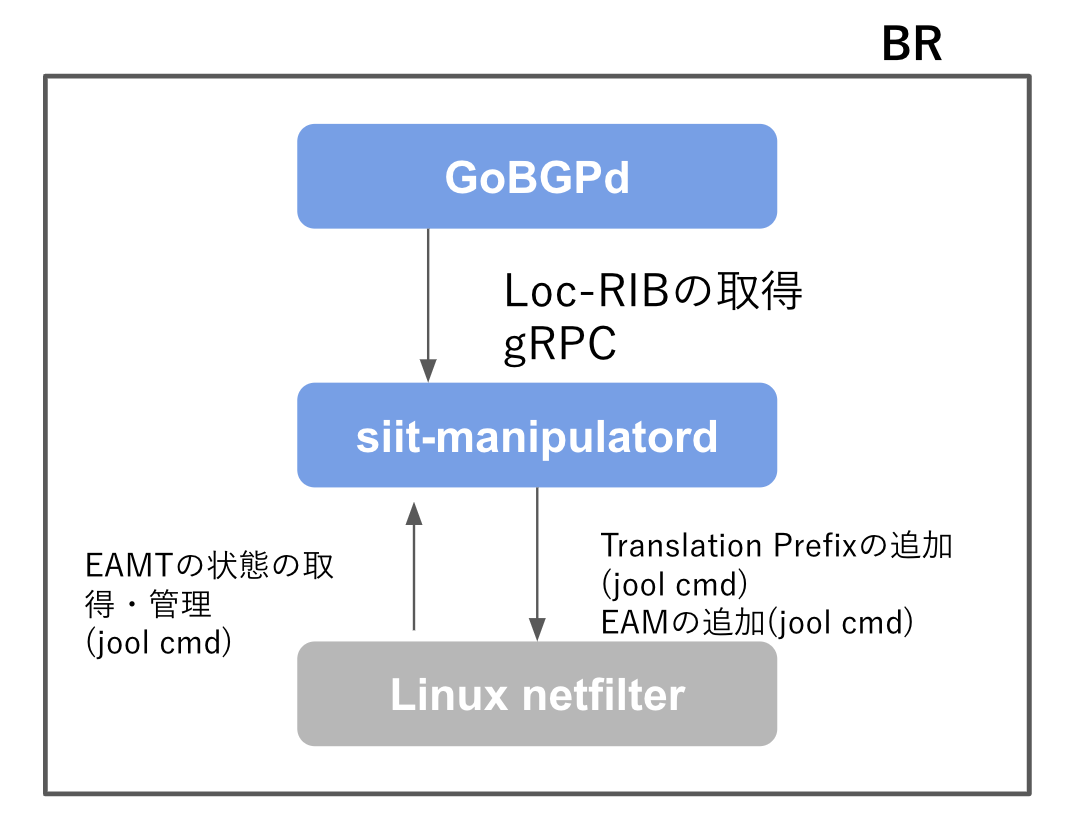
\includegraphics[width=12cm,pagebox=cropbox,clip]{img/poc_implementation.png}
    \end{center}
    \caption{PoCおける各コンポーネントの関係図}
    \label{fig:poc_implementation}
\end{figure}

\subsection{各コンポーネントの実装}
\label{implementation:poc:components}

第\ref{proposal:network:nodes}項で述べたコンポーネントは以下の様にそれぞれ実装した.
BRにおけるコンポーネントの関係を図\ref{fig:poc_implementation}に示す.

\subsubsection{BGPデーモン}
BGPデーモンには,OSSのBGPデーモンであるGoBGP\footnote{\url{https://osrg.github.io/gobgp/}}を利用する.

GoBGPではgRPC\footnote{gRPC Remote Procedure Calls. \url{https://www.grpc.io/}}を用いた操作機構が実装されており,同期・非同期を問わず他のアプリケーションとの連携が容易に行える.
RouteReflector機構もサポートされているため,本PoCでは全てのノードのBGPデーモンとしてこれを利用する.

\subsubsection{SIIT}
SIITにはJool\footnote{Jool. \url{https://jool.mx/en/index.html}}のSIIT モードを利用する.

JoolはLinuxOSで利用できるNAT64/SIIT環境で,Lunux Netfilterによって実装されており,汎用的に様々なプラットフォームでの利用が可能である\cite{JOOL,quintero2016performance}.
EAMTの変更には専用のCLIコマンドを利用する.

\subsubsection{EAMT制御機構}
\label{implementation:poc:siit-manipulatord}
BGP上で受信したLoc-RIBをEAMTに反映するために,EAMT制御機構"siit-manipulatord"を実装した.

gRPCによってGoBGPのLoc-RIBの変化をJoolのCLIコマンドを利用してLinux NetFilter反映するほか、Translation Prefixの定義などSIITに必要な情報を管理する.

%%% Local Variables:
%%% mode: japanese-latex
%%% TeX-master: "./thesis"
%%% End:
